\section{Micro-surgeries on \glsfmtname{cps} Top-level Cells}
\subsection{A Problem}
A \gls{cps} cell can contain an arbitrary number of various objects, like other \gls{ps} variants.  A key difference between \gls{cps} and other variants, however, is that \gls{cps} can use one fixed-size \gls{ruleset} that applies to every possible initial multiset, while other variants typically require the definition of a family of related \glspl{ruleset} that change depending on the problem size n, or even of the specific details and starting state of a given problem instance.

This capacity for fixed-size \glspl{ruleset} is enabled primarily through the use of variables and unification, permitting the rules to adapt to the contents of the cells.  This tends to be an all-or-nothing situation, though, in that a single variable usually matches to the entire contents of whichever cell or \gls{functor} it is specified in.  In the case of two or more variables in the same space, the split of the objects between them is made non-deterministically (per \cref{sec:cps:unification}), and may even be done such that one of the variables is empty.  Anything to be excluded from matching with a variable \emph{must} be listed explicitly, while anything remaining to be excluded from the operation of the rule entirely is covered with the underscore \emph{discard} (aka `don't care') symbol (\(\cpdiscard\)).  This is fine for many cases, but falls short in instances when there will be an unknown quantity of a given object in a cell, and it is not desirable to perform a single operation across all of them as one.

As an example, consider a situation where there are an unknown number of \(d\) objects in the \gls{tlc}, and it is desirable to perform an operation for each of them.  Let there be an \(a\) \gls{functor} containing four \(b\) objects, and a \(c\) \gls{functor} containing three \(d\) objects, \ie{} \(\cpfunc{a}{b^4}\) and \(\cpfunc{c}{d^3}\).  The goal is to write a rule that shall replicate the contents of \(a\) and place them inside a new \(e\) \gls{functor}, and do this once per \(d\) present inside \(c\).  Once completed, \(a\) and \(c\) will hold their original contents from before the execution of the rules.

Intuitively, if this operation is carried out as described, then the ending state of the \gls{tlc} should be that it contains \(\cpfunc{a}{b^4}\), \(\cpfunc{c}{d^3}\) and \(\cpfunc{e}{b^{12}}\).  This \emph{could} be achieved using rules as shown in \cref{rules:cps:slowmulti}.  While this would work, it requires steps equal to the size of the contents of \(c\) plus one (\ie{} four steps), as well as necessitating an uninteresting auxiliary rule.  Minor variations are possible, primarily regarding the choice of use of \glspl{promoter}, \glspl{inhibitor} and states, but ultimately, they would lead to roughly the same set.

\begin{cprulesetfloat}
    \begin{cpruleset}
        \cprule{s_0}{}{\cponce}{s_1}{\cpfunc{e}{\cpempty}~\cpfunc{f}{D}}
        \cppromoter{\cpfunc{c}{D}}
        
        \cprule{s_1}{\cpfunc{c}{dD} \; \cpfunc{e}{E}}{\cponce}{s_1}{\cpfunc{c}{D} \; \cpfunc{e}{EB}}
        \cppromoter{\cpfunc{a}{B}}
    
        \cprule{s_1}{\cpfunc{c}{\cpempty} \; \cpfunc{f}{D}}{\cponce}{s_2}{\cpfunc{c}{D}}
    \end{cpruleset}
    \caption[Simulation of multiplication in cP systems]{\label{rules:cps:slowmulti}Simulation of multiplication in \gls{cps}.  The values in the \(a\) and \(c\) complex terms are multiplied, with the result stored in the \(e\) term.  \Cref{fig:cps:slowmulti} shows a state machine reflecting the rules' progression}
\end{cprulesetfloat}

\begin{figure}
    \centering
    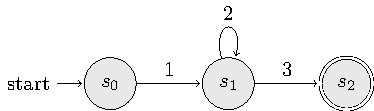
\includegraphics{chapters/cpsystems/ruleset1statemachine.pdf}
    \caption[State machine diagram for the system in \cref{rules:cps:slowmulti}]{State machine diagram for the system in \cref{rules:cps:slowmulti}.  Nodes are labelled with states, and edges with rules transitioning between them}
    \label{fig:cps:slowmulti}
\end{figure}

In particular, it is not possible here to make the second rule work in parallel --- a given \gls{functor} or atom may only be used in one rule application per system step, and so the first rule application would take exclusive control of both the \(c\) \gls{functor} and its \(d\) contents, preventing any further rule applications from occurring.  A further wrinkle of this \gls{ruleset} is the fact that it requires an extra temporary \gls{functor}, \(f\), to store copies of the \(d\) atoms for transfer back into \(c\) at the end because the appropriate termination point for these rules can only be detected when \(c\) has been emptied.

These issues arise because in \gls{cps} only the \glspl{tlc} have computational power.  All nested objects/terms contained within a \gls{tlc} are inert, no matter their level of nesting.  This is unlike most other \gls{ps} variants, where each \gls{compartment} either is elementary (\ie{} has no nesting within itself) or has a separate ruleset, enabling it to evolve independently despite being nested.  Furthermore, when a term is selected on the \gls{lhs} of a rule, it is conceptually deleted at the application of the rule.  If the term is repeated on the \gls{rhs} of the rule, then that is conceptually a new object derived from the old one.

\subsection{A Solution}
To avoid this problem, one may optionally make use of an operation that permits a rule to be applied to the contents of a sub-cell or \gls{functor}, \emph{without} also seizing control (\ie{} locking) of the sub-cell or \gls{functor} itself.  This operation is termed \emph{\gls{ms}}, representing the idea that as-minimal-as-possible (minimally-invasive) modification is made to the containing object while modifying its contents.  \Glspl{ms} are denoted by curly braces, rather than the usual parentheses for complex terms.  They are still complex terms, but the operation performed on them differs.  Due to this differing operation, every instance of a \gls{ms} on the \gls{lhs} \emph{must} have a matching instance on the \gls{rhs}, and they must not appear in \glspl{promoter} or \glspl{inhibitor}.

\begin{cprulesetfloat}
    \begin{cpruleset}
        \cprule{s_0}{}{\cponce}{s_1}{\cpfunc{e}{\cpempty}}

        \cprule{s_1}{\cpfuncms{e}{\,}}{\cpmaxpar}{s_2}{\cpfuncms{e}{B}}
        \cppromoter{\cpfunc{c}{d\cpdiscard}}
        \cppromoter{\cpfunc{a}{B}}
    \end{cpruleset}
    \caption[Rules for destructive multiplication]{\label{rules:cps:microsurg}Rules for a destructive multiplication process that requires exactly two steps regardless of the numbers multiplied by using \gls{cps} \glspl{ms}}
\end{cprulesetfloat}

\Cref{rules:cps:microsurg} is an example of three rules using \glspl{ms} that achieve in \emph{two} steps the same destructive multiplication as \cref{rules:cps:slowmulti}, which requires \(D + 1\) steps.  Crucially, the second rule is still \emph{one} rule application, but the insertion of \(B\) into \(e\) happens once for each possible match on the \gls{promoter}.  The use of \(c(d\cpdiscard)\) combined with the maximally parallel rule mode means that the rule will take control of and execute once for each \(d\) atom in the multiset labelled by the \(c\) \gls{functor}.  As such, three lots of \(B\) will be inserted into \(e\) simultaneously while executing this rule.

Furthermore, destructive division of \(d\) by \(e\), \(d \div e = f\), could be:
\cpruleinline{\cprule*{s_1}{\cpfuncms{f}{\,}~\cpfuncms{d}{E}}{\cpmaxpar}{s_1}{\cpfuncms{f}{\cpundig}~\cpfuncms{d}{\,}~|~\cpfunc{e}{E}}}

Note that in the case of division, the quotient returned in the \(f\) term will be the \emph{floor} of the precise division result, \ie{} the equation could be written as \(\lfloor d \div e \rfloor = f\).  For cases where the dividend is an exact multiple of the divisor, this will be the same as the correct result.  Otherwise, it will be the correct result's whole-number part only.  \Eg{} referring to the rule immediately above, for \(d(6)~\&~e(3)\), the output will be \(f(2)\), whereas for \(d(5)~\&~e(3)\), the output will be \(f(1)\), with the two left-over unary digits remaining in \(d\).  In other words, \(f\) receives the quotient, and \(d\) keeps the remainder.

\lstset{xleftmargin=.5in, xrightmargin=.5in} 
\begin{lstlisting}
  $\cpfuncms{a}{\cpundig} \; \rightarrow_{\cpmaxpar} \; \cpfuncms{a}{B}~|~\cpfunc{b}{B}$ #\hfill\textsl{single-step multiplication}\enspace#
  $\cpfuncms{a}{C} \; \cpfuncms{b}{\,} \; \rightarrow_{\cpmaxpar} \; \cpfuncms{a}{\,} \; \cpfuncms{b}{\cpundig}~|~\cpfunc{c}{C}$ #\hfill\textsl{single-step floor division}\enspace#
\end{lstlisting}